\subsection{Circadian entrainment phase: Towards a unified mathematical
model}

The perfect coordination of the oscillation periods between the
behaviour and the environment is not the only phenomenon in
chronobiology. Those periods can be perfectly aligned, but the
relative phase of this alignment, or the entrainment phase, is a no
less important feature of circadian entrainment and has been focus of
research for many decades, see, for
instance,~\cite{pittendrigh1981circadian}. Within this project, we
attempted to describe the behaviour of the entrainment phase in as
simple a mathematical model as possible and to uncover some common
patterns of its reaction to changes in the environment.

\subsubsection{Human chronotypes and the 180 degree rule}
A first striking example of the apparent unpredictability of
entrainment phase is the discrepancy between how precise our clocks
are in terms of the internal period and how broadly distributed are
our wake-up times. The reported precision of the clock is within a
quarter of hour, whereas the wake-up times (as a proxy of entrainment
phase) has a characteristic deviation of two hours across human
population \cite{duffy2005entrainment}. If our clocks are so precise,
why are our alarms not so?

We explained this disproportion between the period and phase precision
by recognizing the so-called 180-degree rule~\cite{granada2013human}.
The rule asserts that within a population with a however broad or
narrow distribution of internal periods $\tau$, distribution of phases
of entrainment as broad as 180 degrees are inevitable. Moreover, the
width of the entrainment range of the subject determines the
sensitivity of the entrainment phase to the mismatch between the
period $T$ of entraining environment (usually 24 hours) and the
internal period $\tau$.

The explanation for the 180 degree rule is based on the inspection of
the structure of entrainment range in the simplest oscillator models.
The phase of entrainment assumes maximal and minimal values at the
borders of entrainment range and the those values span an interval of
180 degrees. Now if the oscillator is easily entrainable (or ``weak''
as we call it), it has a wide entrainment range in terms of tolerated
mismatches between $\tau$ and $T$ and small changes in $\tau-T$ (by
changing $\tau$ for example across the population) are translated in
relatively small changes of entrainment phase. If, on the other hand,
the oscillator is ``strong'', i.e. it entrainment range is narrow in
terms of $\tau-T$, small changes in $\tau$ would be translated in
large changes of entrainment phase. Given the precision of circadian
rhythms in mammals, including humans, it is thus no surprise that
a narrow distribution of $\tau$ across the population causes a broad
distribution of entrainment phases aka wake-up times.

\begin{figure}
\begin{center}
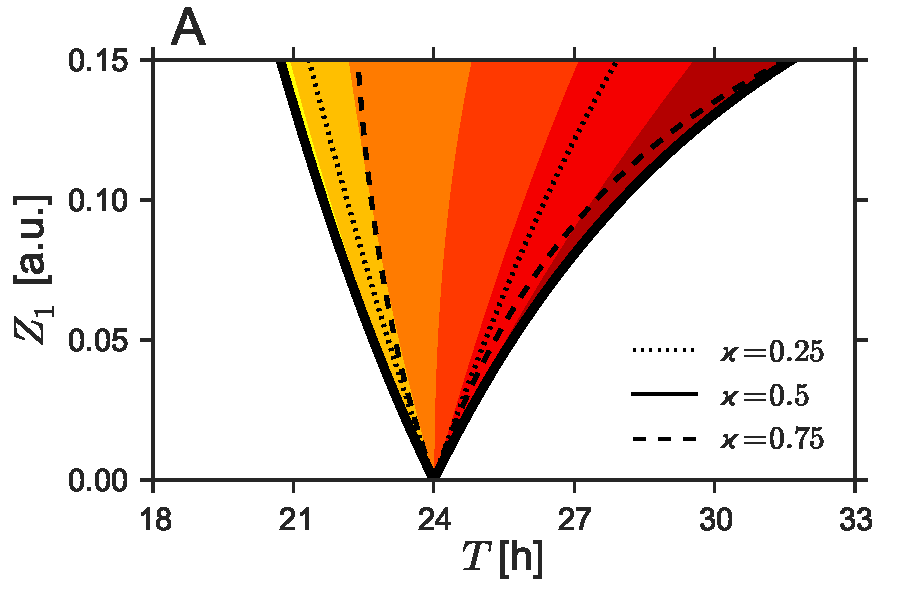
\includegraphics[width=0.49\linewidth]{figures/phase/fig1A.pdf}
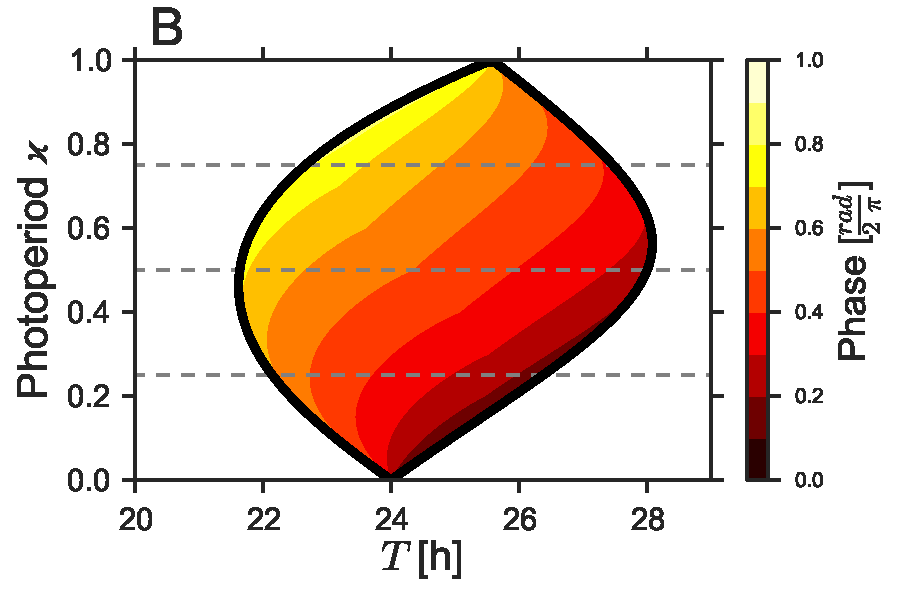
\includegraphics[width=0.49\linewidth]{figures/phase/fig1B.pdf}
\end{center}
\caption{
  {\bf A} Dependence of phase of entrainment within an Arnold tongue
  on Zeitgeber period $T$ and strength $Z_1$ for different
  photoperiods $\chi$.
  {\bf A} Dependence of phase of entrainment within an onion-like
  region on Zeitgeber period $T$ and photoperiod $\chi$.
\label{fig::phase}
}
\end{figure}

\subsubsection{Phase of entrainment in seasonality}
